\documentclass[11pt]{report}

\usepackage[final]{graphicx}
\usepackage{indentfirst}
\usepackage{url}
\usepackage{cite}

\textwidth = 6.5 in
\textheight = 9 in
\oddsidemargin = 0.0 in
\evensidemargin = 0.0 in
\topmargin = 0.0 in
\headheight = 0.0 in
\headsep = 0.0 in
\parskip = 0.0 in
\parindent = 0.4 in

\begin{document}

\newcommand{\sect}[1]{\section*{\center #1}}
\renewcommand{\abstractname}{\Large \textbf{Abstract}}
\renewcommand{\bibname}{\center \Large \textbf{References}}
\renewcommand{\contentsname}{\center \Large \textbf{Table of Contents}}

\begin{titlepage}

\vspace*{0.5in}
\begin{center} \LARGE A \LaTeX\ Driver for the FreeHEP VectorGraphics Framework\\[26pt]
\normalsize
Andre Bach\\[6pt]
Reed College\\[26pt]
Student Undergraduate Laboratory Internship (SULI)\\[6pt]
Stanford Linear Accelerator Center (SLAC)\\[6pt]
Stanford, California\\[26pt]
August 20, 2004
\end{center}
\vspace{39pt}
\setlength{\baselineskip}{19pt}

Prepared in partial fulfillment of the requirements of the Office of Science, Department of Energy's Science Undergraduate Laboratory Internship under the direction of Mark D\"onszelmann in the Computing Services Department at the Stanford Linear Accelerator Center.
\vspace{32pt}
\begin{tabbing}
Research Advisor:~~ \= \underline{\hspace{2in}}\kill
Participant: \> \underline{\hspace{2in}}\\[39pt]
Research Advisor: \> \underline{\hspace{2in}}
\end{tabbing}
\end{titlepage}

\setlength{\baselineskip}{26pt}

\tableofcontents
\thispagestyle{empty}

\begin{abstract}
\addcontentsline{toc}{section}{Abstract}
A \LaTeX\ Driver for the FreeHEP VectorGraphics Framework. ANDRE BACH (Reed College, Portland, OR 97202) MARK D\"ONSZELMANN (Stanford Linear Accelerator Center, Stanford, CA 94025)

\vspace{13pt}
\noindent
The FreeHEP library is the ongoing project of an open source collaboration to create and share Java code in high energy physics and other fields. One component of FreeHEP is the VectorGraphics framework, which enables the export of graphics to a wide variety of formats beyond Java's basic capabilities. This paper describes an addition to VectorGraphics, a driver for the \LaTeX\ PSTricks package. \LaTeX\ is a markup language in wide use by physicists and others for producing academic papers for publication. PSTricks is an extension of \LaTeX\ that provides PostScript macros allowing complicated vector graphics to be written directly into \LaTeX\ code. The ability to export graphics directly to a \LaTeX\ native format will ease their inclusion into such documents. The context of FreeHEP and VectorGraphics into which this driver fits is described. All the main functionality of the driver is in place, but some limitations remain. Some details of its construction, as well as outstanding problems, are addressed.
\end{abstract}

\setcounter{page}{1}
\sect{Introduction}
\addcontentsline{toc}{section}{Introduction}

High energy physics is one of the most successful and spectacular of the sciences. At the Stanford Linear Accelerator Center, a few of the many areas of research are the investigation of CP Violation, the subtle difference between the laws governing matter and antimatter; the characterization of many different materials using synchrotron radiation; and the construction of GLAST, a satellite that will provide unprecedented clarity in gamma ray astronomy. All this requires considerable support structure, both physical and computational. FreeHEP is an open source Java library of various components and other programs that are of use in both high energy physics and other fields \cite{fhep:web, fhep:talk1, fhep:talk2}. FreeHEP contains packages for, among other things, high energy physics data analysis and event display, a framework for Java applications, and the subject of this paper, VectorGraphics, an extension of the graphics capabilities of the standard Java libraries.

The experiments of high energy physics invite the use of graphics and visualization. Besides the graphs and plots common to all sciences, high energy physics also features large detectors and intricate collisions that must be assessed visually in order to properly work with and appreciate the data and experiments. These graphics, then, must be included in academic papers and many other communications. This necessitates a means of exporting graphics from the various programs used in high energy physics to formats compatible with the different types of documents in which they will be included. The core Java graphics libraries \cite{java:api} cannot accomplish this, as they output only bitmaps, which are ill suited for scaling and other common manipulations. Graphics formats fall into two categories, bitmap and vector. In a bitmap graphic, a color is specified for each pixel in a way analogous to photographic film, making it inappropriate for highly ordered line graphics such as graphs. Vector graphics are specified in terms of the lines and curves that appear in the picture and thus scale perfectly while frequently requiring less disk space. The VectorGraphics package of the FreeHEP library is an extension of the Java graphics system that enables programs used in physics and other fields to export graphics to a wide variety of formats, fulfilling the need.

The goal is to create and test an addition to VectorGraphics, a driver for outputting vector graphics in a \LaTeX\ format, suitable for direct inclusion in a \LaTeX\ document. \LaTeX, a more user-friendly extension of \TeX, is a markup language in wide use in the physical sciences and other areas. Markup languages (of which HTML is another example) are used to format text by entering the text along with commands specifying font, text size, and all other attributes into a source file which is then compiled to produce the final document. \LaTeX\ allows authors to easily achieve near-professional quality typesetting themselves with minimal intervention from journal editors, increasing the speed and ease of publishing and allowing documents created by those with minimal typographical skill to appear professionally produced. It is especially popular for its powerful formatting of mathematical equations. Currently, the most common method for including graphics in \LaTeX\ documents is to produce a stand alone graphics (e.~g., PostScript) file and provide a reference command to it in the \LaTeX\ source code along with information specifying the location and size of the graphic in the document \cite{kopka, hoenig}. A driver for writing vector graphics directly to \LaTeX\ code for inclusion into the \LaTeX\ source of a document will ease the inclusion of graphics in documents produced by \LaTeX. This will be of use to both the high energy physics community and the many other users of \LaTeX. A further benefit is the ease with which those already familiar with \LaTeX\ can hand-edit the graphics code for fine control and changes to the images, something far more difficult with the more esoteric PostScript code.

\sect{Java and FreeHEP}
\addcontentsline{toc}{section}{Java and FreeHEP}

FreeHEP is an open source project, open to all for use or modification. This aids high energy physics and other fields by minimizing duplication of effort and allowing widely dispersed groups to build on each other's work. The vast majority of FreeHEP is written in Java code. The primary benefit of using Java is its cross-platform compatibility. In most programming languages, the source code is compiled to the machine-readable code that is actually run by the computer. Since each platform has very different machine code, this makes it difficult to port programs from one system to another. Java source code, on the other hand, is always compiled to code readable by the Java Virtual Machine. When a Java program is run, the computer runs the JVM, and the JVM runs the program and relays its commands to the computer in the appropriate platform-specific language. Thus, Java programs will run on any platform for which a JVM has been written, practically all of them.

A further benefit of Java is that it is an object oriented programming language. This means that the code for a project is divided into smaller units, called classes, that can interact with each other in various ways. This allows the FreeHEP libraries to be both modular and easily expandable. Each graphics driver, for instance, is a different implementation of the same superclass. This eliminates redundancy because all the code common to all drivers is written just once, in the superclass, and makes it easy to determine exactly what a new driver must do. Finally, we feel that several technical features of Java, such as not needing to manually deal with memory leaks, make programming with it more efficient and rewarding. 

Several of the components of the FreeHEP library and related projects produce graphics that authors may want to include in their papers. JAS3, a data analysis tool, outputs histograms, scatter plots, and other graphs \cite{jas3:web}. WIRED, a framework for the visualization of high energy physics events, outputs displays of detectors and particle paths \cite{bal, wired:web}. There are, in addition, many more components of FreeHEP that do not have a direct bearing on graphics. This project is part of the VectorGraphics portion of FreeHEP, which enables the other FreeHEP programs to export graphics to a wide array of formats. Because of the minimal interdependence of the FreeHEP libraries, outside developers can also freely use VectorGraphics for their programs without using the rest of FreeHEP\@.

The VectorGraphics package has a somewhat complex structure of classes, illustrated in Figure~1. \begin{figure}[tb] \hspace{.6in} 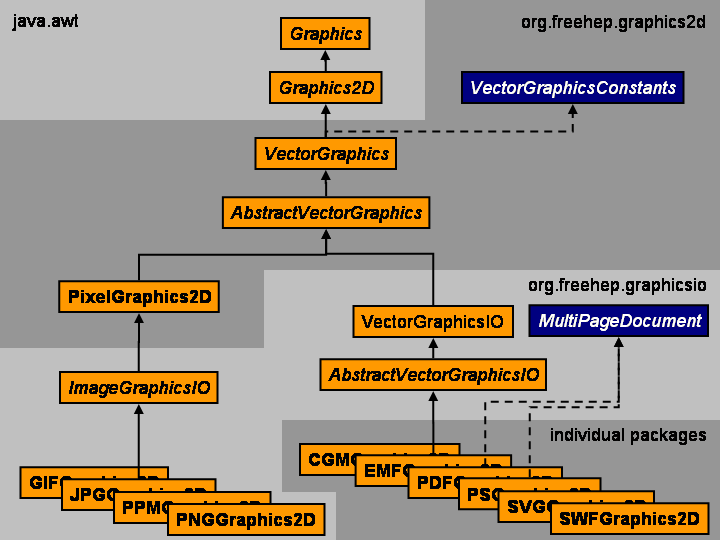
\includegraphics[scale=1]{ClassDiagram2} \caption{Diagram of VectorGraphics class structure.} \end{figure} \addcontentsline{toc}{subsection}{Figure 1: VectorGraphics class structure.} The Graphics and Graphics2D classes are part of the standard Java installation used by everyone. VectorGraphics and AbstractVectorGraphics redefine the standard methods and add additional methods. VectorGraphicsIO and AbstractVectorGraphicsIO provide additional methods and an outline for specific vector graphics drivers. The core of this project, LatexGraphics2D, is another entry at the bottom right of the figure, joining the other individual packages. Running parallel to the illustrated class structure are the support classes that handle specific tasks. Most important of these are the PathConstructors, which manage the drawing of lines and curves. 

\sect{Implementation of the Driver}
\addcontentsline{toc}{section}{Implementation of the Driver}

The basic task of a graphics driver such as this one is to convert the information of a graphic from the form it exists as within a program into a specific file type that can be written to disk, in this case \LaTeX. The information comes to the driver in the form of method calls. That is, if the color is to be set to blue, a section of code named \texttt{writePaint(...)} will be called with the color blue as its argument. The output is one file of a linear sequence of commands that can be interpreted by the \LaTeX\ compiler to produce the actual picture again and are also human readable and editable. Standard \LaTeX\ has only very limited capabilities for producing graphics, so for writing graphics to \LaTeX\ it is necessary to use an extension that includes all the standard graphics commands. Originally we considered pict2e, an extension of the standard \textsf{picture} environment, but we found its capabilities to be too limited \cite{pict}. Another \LaTeX\ extension, PSTricks \cite{zandt}, was found to be suitably comprehensive. PSTricks allows most PostScript commands to be written into \LaTeX\ files by way of user-friendly macros, though it does have some limitations.

Any driver extending the Java Graphics2D class has a number of methods that it must implement, a list that is further extended by the VectorGraphics superclasses. The starting point in creating a new VectorGraphics driver is a class called DummyGraphics2D. This contains declarations of all the required methods along with brief descriptions of what each is supposed to do, a very useful tool given the large number of methods to be implemented. While this forms the basis of LatexGraphics2D, the core of the driver, two other components, LatexPathConstructor and LatexExportFileType, also had to be created. This structure is shared with all the VectorGraphics drivers, some of which have many more secondary classes. Frequently the most useful technique when uncertain about some aspect of the program is to look at how that same aspect was handled in the many other drivers that are already written.

One example of code and the output produced is provided to illustrate the operation of the driver. Suppose that the picture contains a triangle. This is stored as an object with specifications of where the vertices are located. The first piece of code in LatexGraphics2D called to draw the triangle is \texttt{draw(...)}: \newpage
\setlength{\baselineskip}{13pt}
\begin{verbatim}
public void draw(Shape shape) {
    LatexPathConstructor pc = new LatexPathConstructor(ps);
    try {
        ps.println("\\pscustom[fillstyle=none]{");
        pc.addPath(shape, getTransform());
        ps.println("}");
    } catch (IOException e) {
        handleException(e);
    }
}
\end{verbatim}
\setlength{\baselineskip}{26pt} \vspace{-10pt}
The code above writes the beginning of a pscustom environment, in which all objects are drawn, to the printstream \texttt{ps} that will become the file. It then passes the shape to a new PathConstructor \texttt{pc}, which writes the code for that shape. After it finishes that, the pscustom environment is ended. Breaking the shape down into its components is the same for all formats and so is handled by the PathConstructor superclasses. When that is done, methods in LatexPathConstructor write the lines and other components of the triangle. One such method is \texttt{line()}:

\setlength{\baselineskip}{13pt}
\begin{verbatim}
public void line(double x, double y) throws IOException {
    ps.println("\\lineto("+fixedPrecision(x)+","+fixedPrecision(y)+")");
}
\end{verbatim}
\setlength{\baselineskip}{26pt} \vspace{-10pt}
This simply writes a command specifying that a line be drawn from whatever the current point is to the point $x,y$. Other methods for drawing curves and moving the current point are similar. The final output for a triangle might look like this:

\setlength{\baselineskip}{13pt}
\begin{verbatim}
\pscustom[fillstyle=none]{
    \moveto(300.0,388.105117)
    \lineto(267.0,330.947441)
    \lineto(333.0,330.947441)
    \closepath
}
\end{verbatim}
\setlength{\baselineskip}{26pt} \vspace{-10pt}
This PSTricks \LaTeX\ code creates a triangle by moving to a certain point, drawing a line from that point to another, drawing a second line from the endpoint of the first line to a third point, and then closing the path, which draws a line from the last point to the point that was the argument of \verb=\moveto=. The true visible lines are actually drawn (``stroked'') only at the end of the pscustom environment, which allows the line joins to be drawn properly.

The VectorGraphics drivers are tested by means of about thirty test files, small Java programs that produce images to test specific aspects of a graphics driver. The simplest of these, TestLineStyles, is shown in Figure~2. \begin{figure}[tb] \hspace{1.5in} 
\includegraphics[scale=0.4]{TestLineStyles} \caption{Output of TestLineStyles.} \end{figure} \addcontentsline{toc}{subsection}{Figure 2: TestLineStyles} The primary means of writing the driver is to attempt to implement some feature, run the appropriate test file, see if it is drawn correctly, fix the code, and repeat as necessary.

An additional test class, TestGraphicsContexts, was written for this project. From the point of view of the Java program, graphics are drawn in graphics contexts, each with different style specifications such as current color and line width. In Java, these contexts can be nested within each other, but since the output file is linear, the style specifications must be saved when a context is exited and restored when it is re-entered. TestGraphicsContexts was created to ensure that this process was handled correctly.

The major features of the driver are all in place, but there are some limitations and room for future work. In a few cases, text appears misplaced. Text cannot be resized by the same mechanism as the rest of the image. The files that are currently created are stand alone \LaTeX\ files and must have their headers deleted by hand to be included in other \LaTeX\ files; there should be an option in the save as dialog to save as a stand alone file or not. These files may be included in other \LaTeX\ files by using the \verb=\input{=\textsl{file}\verb=}= command as the \verb=\includegraphics{=\textsl{file}\verb=}= command would be used. Some limitations are due to PSTricks, which does not currently support a number of features such as line join styles or repeating gradients. Further details on the limitations may be found in the FreeHEP API \cite{fhep:api}.

\sect{Conclusion}
\addcontentsline{toc}{section}{Conclusion}

A driver was created using the FreeHEP VectorGraphics framework that allows any Java program using the VectorGraphics package to export graphics to a \LaTeX\ file using the PSTricks extension. The driver has several limitations, which are documented.

\sect{Acknowledgements}
\addcontentsline{toc}{section}{Acknowledgements}

I thank the Department of Energy and the Stanford Linear Accelerator Center for creating, organizing, and funding the Summer Undergraduate Laboratory Internship program, which made this project possible. I also thank my mentor, Mark D\"onszelmann, for all his help. Finally, thank you to all the other participants in the program for making it so interesting.


\setlength{\baselineskip}{13pt}
\bibliographystyle{IEEEtran}
\bibliography{Latexbibdata}
\addcontentsline{toc}{section}{References}

\end{document}